\documentclass{article}

\usepackage{amsmath}
\usepackage{amssymb}
\usepackage{parskip}
\usepackage{fullpage}
\usepackage{hyperref}
\usepackage{tikz}
\usepackage{float}

\hypersetup{
    colorlinks=true,
    linkcolor=black,
    urlcolor=blue,
    pdftitle={Differentiation},
    pdfpagemode=FullScreen,
}

\title{Differentiation}
\author{Paolo Bettelini}
\date{}

\begin{document}

\maketitle
\tableofcontents
\pagebreak

\section{Definition}

\subsection{Tangent}

\begin{minipage}{0.5\textwidth}
    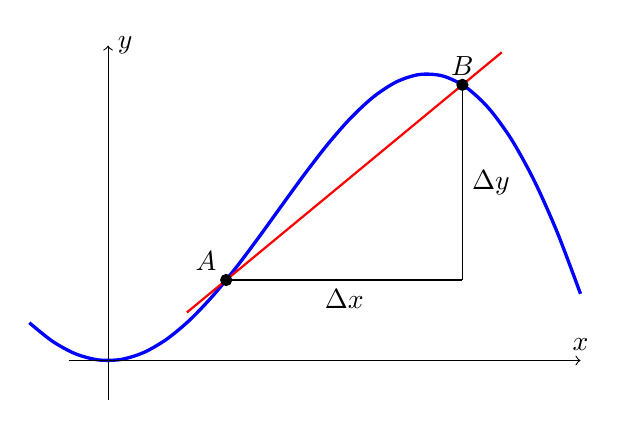
\begin{tikzpicture}[
        scale=2,
        declare function={
            func(\x) = \x*sin(\x r);
            Width=3;
            Height=2;
            Ax=0.75;
            Bx=2.25;
            SlopeMargin=0.25;
            M=(func(Bx) - func(Ax)) / (Bx - Ax);
            Q=func(Ax) - M * Ax;
            slopeFunc(\x)=\x * M + Q;
        }
    ]
        \draw[domain=-0.5:3, smooth, variable=\x, blue, very thick] plot ({\x}, {func(\x)});
        
        \draw[->] (0, -0.25) -- (0, Height) node[right] {\(y\)};
        \draw[->] (-0.25, 0) -- (Width, 0) node[above] {\(x\)};

        \draw[-] (Ax, {func(Ax)}) -- node[below] {\(\Delta x\)} (Bx, {func(Ax)});
        \draw[-] (Bx, {func(Ax)}) -- node[right] {\(\Delta y\)} (Bx, {func(Bx)});
        
        \filldraw [red, thick] ({Ax - SlopeMargin}, {slopeFunc(Ax - SlopeMargin)}) -- ({Bx + SlopeMargin}, {slopeFunc(Bx + SlopeMargin)});
        
        \filldraw [black] (Ax,{func(Ax)}) circle (1pt) node[above left] {\(A\)};
        \filldraw [black] (Bx,{func(Bx)}) circle (1pt) node[above] {\(B\)};
    \end{tikzpicture}
\end{minipage}
\begin{minipage}{0.5\textwidth}
    The mean slope of a function \(f\) between a point \(A\) and \(B\) is given by
    \[
        \frac{\Delta y}{\Delta x} = \frac{f(B)-f(A)}{B-A}
    \]
    As we make \(A\) and \(B\) closer to eachother, \(\Delta x\) decreases.
    As \(\Delta x\) decreases the mean slope is more representative of the rate of change
    of \(f\) in the interval \([A;B]\). \\
\end{minipage}

\begin{minipage}{0.5\textwidth}
    When \(\Delta x\) is infinitely small, we have the precise slope of a given point
    on the function. This slope is represented by the tangent line, which is parallel to the given point.
    \[
        \lim_{\Delta x \to 0} \frac{\Delta x}{\Delta x}
    \]
\end{minipage}
\begin{minipage}{0.5\textwidth}
    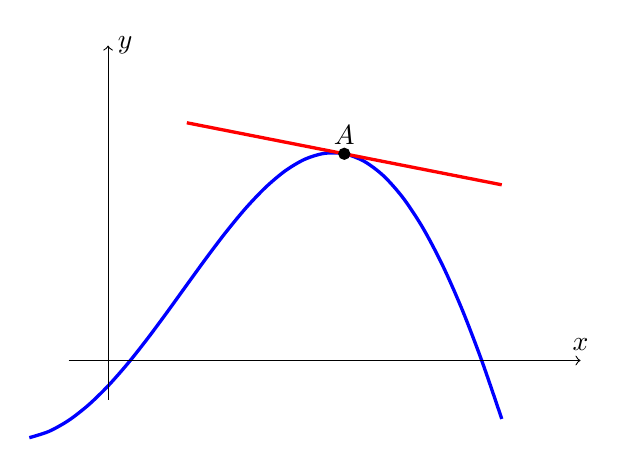
\begin{tikzpicture}[
        scale=2,
        declare function={
            func(\x) = (\x+0.6)*sin((\x+0.6) r)-0.5;
            Width=3;
            Height=2;
            Ax=1.5;
            slope = -0.19697;
        }
    ]
        \draw[domain=-0.5:2.5, smooth, variable=\x, blue, very thick] plot ({\x}, {func(\x)});
        
        \draw[->] (0, -0.25) -- (0, Height) node[right] {\(y\)};
        \draw[->] (-0.25, 0) -- (Width, 0) node[above] {\(x\)};

        \draw[domain=0.5:2.5, smooth, variable=\x, red, very thick] plot ({\x}, {slope * \x + func(Ax) - slope * Ax});
        
        \filldraw [black] (Ax,{func(Ax)}) circle (1pt) node[above] {\(A\)};
    \end{tikzpicture}
\end{minipage}

\subsection{Derivative}

The derivative of a function \(f(x)\) is another function \(f'(x)\) which
represents the rate of change of \(f(x)\). In other words, \(f'(x)\)
represents the slope at each \(x\) of \(f(x)\).

We define \(f'(x)\) by taking the limit of the slope for every \(x\).

\begin{minipage}{0.5\textwidth}
    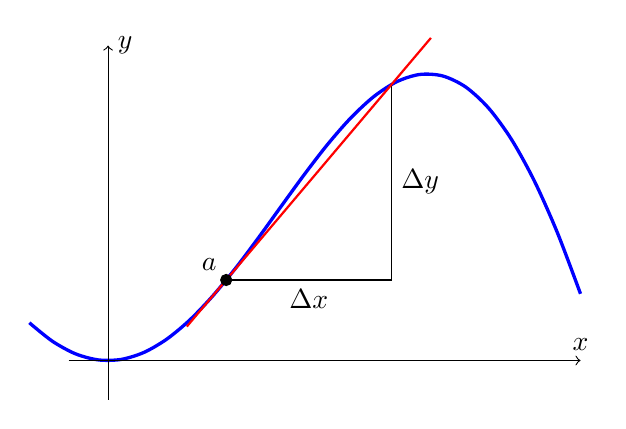
\begin{tikzpicture}[
        scale=2,
        declare function={
            func(\x) = \x*sin(\x r);
            Width=3;
            Height=2;
            Ax=0.75;
            Bx=1.8;
            SlopeMargin=0.25;
            M=(func(Bx) - func(Ax)) / (Bx - Ax);
            Q=func(Ax) - M * Ax;
            slopeFunc(\x)=\x * M + Q;
        }
    ]
        \draw[domain=-0.5:3, smooth, variable=\x, blue, very thick] plot ({\x}, {func(\x)});
        
        \draw[->] (0, -0.25) -- (0, Height) node[right] {\(y\)};
        \draw[->] (-0.25, 0) -- (Width, 0) node[above] {\(x\)};

        \draw[-] (Ax, {func(Ax)}) -- node[below] {\(\Delta x\)} (Bx, {func(Ax)});
        \draw[-] (Bx, {func(Ax)}) -- node[right] {\(\Delta y\)} (Bx, {func(Bx)});
        
        \filldraw [red, thick] ({Ax - SlopeMargin}, {slopeFunc(Ax - SlopeMargin)}) -- ({Bx + SlopeMargin}, {slopeFunc(Bx + SlopeMargin)});

        \filldraw [black] (Ax,{func(Ax)}) circle (1pt) node[above left] {\(a\)};
    \end{tikzpicture}
\end{minipage}
\begin{minipage}{0.5\textwidth}
    We define the derivative as
    \[
        f'(x) = \lim_{\Delta x \to 0} \frac{f(x + \Delta x) - f(x)}{\Delta x}
    \]
    or
    \[
        f'(x) = \lim_{h \to x} \frac{f(h) - f(x)}{x-h}
    \]
\end{minipage}

\begin{itemize}
    \item If \(f'(a) > 0\), then \(f(x)\) is increasing at \(x=a\)
    \item If \(f'(a) < 0\), then \(f(x)\) is decreasing at \(x=a\)
    \item If \(f'(a) = 0\), then \(f(x)\) is critical at \(x=a\) (changing from increase to decrease or from decrease to increase)
\end{itemize}

\pagebreak

\section{Chain Rule}

\subsection{Definition}

If \(z\) depends on \(y\), and \(y\) depends on \(x\), then \(z\) also depends on \(x\).

\[
    \frac{dz}{dx}=\frac{dz}{dy}\cdot\frac{dy}{dx}
\]

\subsection{Proof}

Assuming that \(z\) and \(y\) are differentiable in \(x\)

\begin{align*}
    \frac{dz}{dx}
    &= \lim_{\Delta x \to 0} \frac{\Delta z}{\Delta x}
    = \lim_{\Delta x \to 0} \frac{\Delta z}{\Delta y} \cdot \frac{\Delta y}{\Delta x} \\
    &= \left(
        \lim_{\Delta x \to 0} \frac{\Delta z}{\Delta y}
    \right)
    \left(
        \lim_{\Delta x \to 0} \frac{\Delta y}{\Delta x}
    \right) \\
    &= \left(
        \lim_{\Delta x \to 0} \frac{\Delta z}{\Delta y}
    \right)
    \cdot
    \frac{dy}{dx}
\end{align*}

As \(\Delta x \to 0\) also \(\Delta y \to 0\), so we can replace \(\Delta x\) with \(\Delta y\)

\begin{align*}
    \frac{dz}{dx}
    &= \left(
        \lim_{\Delta y \to 0} \frac{\Delta z}{\Delta y}
    \right)
    \cdot
    \frac{dy}{dx} \\
    &= \frac{dz}{dy} \cdot \frac{dy}{dx}
\end{align*}

\pagebreak

\section{Rules for differentiation}

\[
    \frac{d}{dx}(n)=0
\]

\[
    \frac{d}{dx}(x^n)=nx^{n-1},\quad n\in\mathbb{R}^*
\]

\[
    \frac{d}{dx}\left(n\cdot f(x)\right)=n\frac{d}{dx}\left(f(x)\right)
\]

\[
    \frac{d}{dx}(f+g)=f'+g'
\]

\[
    \frac{d}{dx}(f\cdot g)=g'f+gf'
\]

\[
    \frac{d}{dx}(f(g(x)))=f'(g(x))\cdot g'(x)
\]

\[
    \frac{d}{dx}(f^g)=f^g\left(\frac{f'g}{f}+g'\ln f\right)
\]

\end{document}
